\documentclass[c]{beamer}

\usepackage[utf8]{inputenc}
\usepackage[french]{babel}

\usepackage{amsfonts}
\usepackage{amsmath}

\newtheorem*{deffr}{Définition}
\newtheorem*{propriete}{Propriété}
\newtheorem*{theofr}{Théorème}

\usepackage{graphicx}

\usetheme{Warsaw}

\title{Dynamique d'un graphe}
\author{Igor Colin}
\date{\today}

\setbeamertemplate{navigation symbols}{}

\AtBeginSection[]
{
    \begin{frame}<beamer>
        \tableofcontents[currentsection]
    \end{frame}
}

\begin{document}

\maketitle

\section{Données à disposition}
\begin{frame}
    \begin{columns}
        \begin{column}{.5\textwidth}
            \begin{itemize}
                \item<1-> Données de départs : graphe utilisateurs
                \item<2-> N\oe{}uds : utilisateurs
                \item<3-> Arrêtes :
                    \begin{itemize}
                        \item<3-> relations d'amitié
                        \item<4-> influence
                        \item<5-> fréquence de partage
                    \end{itemize}
            \end{itemize}
        \end{column}
        \begin{column}{.5\textwidth}
            \only<2>{
                \begin{figure}
                    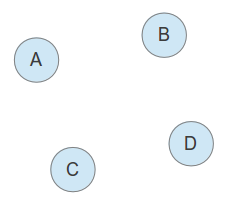
\includegraphics[width=.7\textwidth]{./figures/users.png}
                \end{figure}
            }
            \only<3>{
                \begin{figure}
                    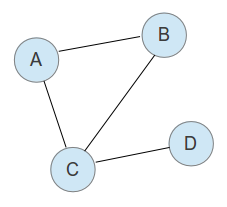
\includegraphics[width=.7\textwidth]{./figures/users_friendship.png}
                \end{figure}
            }
            \only<4>{
                \begin{figure}
                    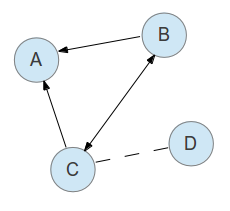
\includegraphics[width=.7\textwidth]{./figures/users_influence.png}
                \end{figure}
            }
            \only<5>{
                \begin{figure}
                    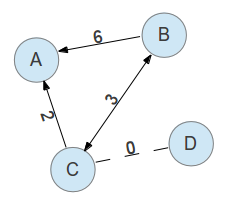
\includegraphics[width=.7\textwidth]{./figures/users_frequency.png}
                \end{figure}
            }
        \end{column}
    \end{columns}
\end{frame}

\begin{frame}
    Plusieurs objectifs :
    \begin{itemize}
        \item Obtenir les paramètres du graphe (influence, sémantique)
        \item Comprendre la structure du graphe (communautés, dynamique)
        \item Agir sur le graphe
    \end{itemize}
\end{frame}

\section{Détection de communautés}
\begin{frame}

    \begin{itemize}
        \item Définition d'une mesure de qualité d'une partition d'un
        graphe
        \item Maximisation de cette quantité pour trouver la partition
        optimale

        \begin{figure}
            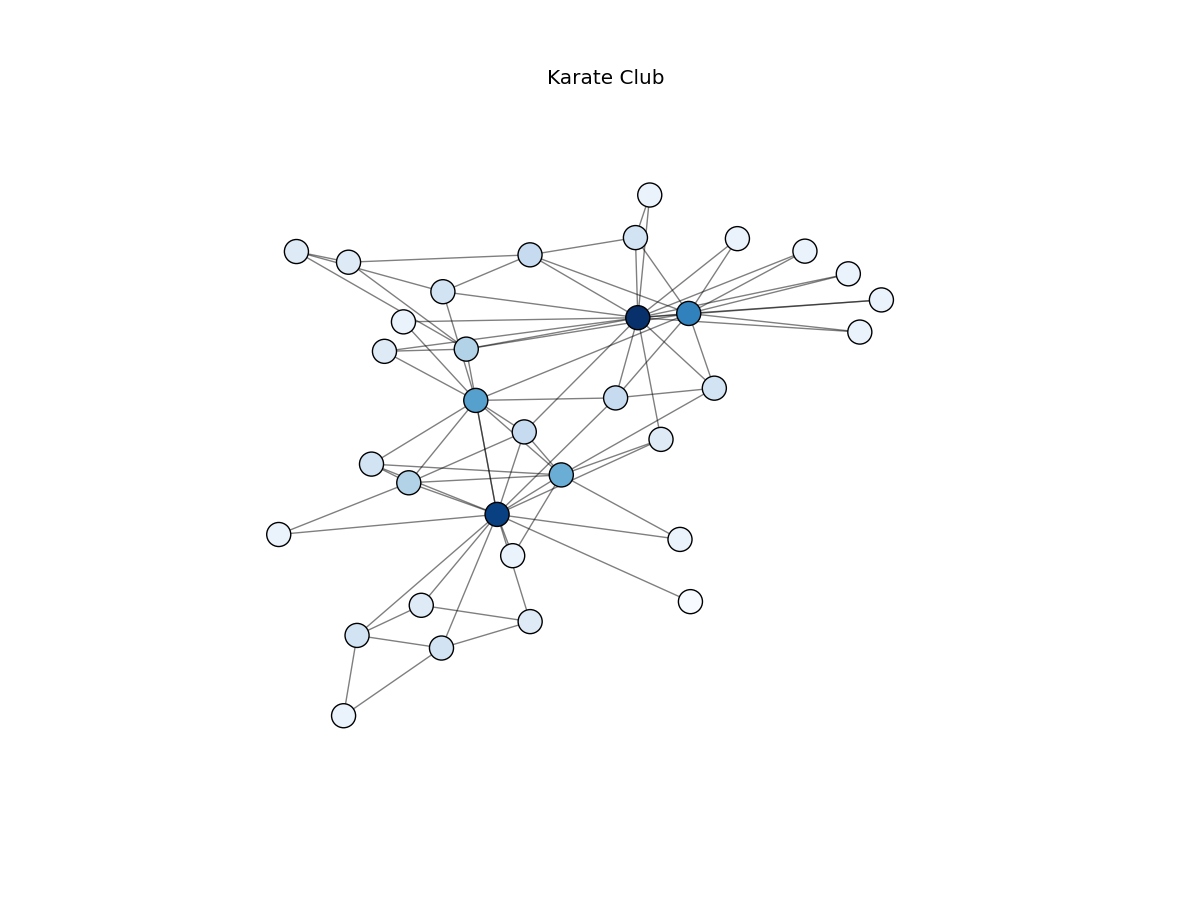
\includegraphics[width=.6\textwidth]{./figures/karate_club.png}
            \caption{Exemple du club de karaté de Zachary.}
        \end{figure}
    \end{itemize}
\end{frame}

\begin{frame}
    \frametitle{Approche spectrale}
    \begin{itemize}
        \begin{deffr}
            Soit $G = (V, E)$ un graphe non-orienté et soit $(S, T)$ une
            partition de $V$. La modularité associée à la partition $(S, T)$
            correspond taux d'arrêtes de $E$ contenues dans $S$ ou $T$ comparé
            au taux d'arrêtes qui auraient été contenues dans $S$ ou $T$ si
            l'on avait distribué les arrêtes du graphe aléatoirement.
        \end{deffr}

        \item Définition de la modularité dépendantes de l'aléa autorisé sur
        les arrêtes
        \item Approche usuelle : degrés des n\oe{}uds conservés
    \end{itemize}

\end{frame}

\begin{frame}
    \frametitle{Approche spectrale}
    \begin{deffr}
        Soit $G = (V, E)$ un graphe non-orienté et soit $(S, T)$ une partition
        de $V$. On note $\mathbf{A}$ la matrice d'adjacence associée à $G$.
        Sous les conditions précédentes, la modularité $Q(S, T)$ peut-être
        exprimée sous la forme suivante :
        \[
            Q(S, T) = \frac{1}{2|E|} \sum_{(i, j) \in V \times V}
                \left( A_{ij} - \frac{d_i d_j}{2|E|} \right)
                \mathbf{1}_{\{s_i = s_j\}},
        \]
        où, pour tout $k \in V$,
        \[
            s_k = \left\{
                \begin{array}{ll}
                    +1 & \text{si $k \in S$} \\
                    -1 & \text{si $k \in T$}
                \end{array}
            \right.
        \]
    \end{deffr}

\end{frame}

\begin{frame}
    \frametitle{Approche spectrale}

    \begin{theofr}
        Soit $G = (V, E)$ un graphe non-orienté. Soit $\mathbf{u^{(2)}}$ le vecteur
        propre associé à la deuxième plus grande valeur propre $\lambda^{(2)}$
        de la matrice de Laplace normalisée. Si $\lambda^{(2)} > 0$, alors la
        partition $(S, T)$ définie par :
        \[
            \left\{
                \begin{array}{r c l}
                    S & = & \{ i \in V \text{, } u^{(2)}_i > 0 \} \\
                    T & = & \{ i \in V \text{, } u^{(2)}_i \leq 0 \}
                \end{array}
            \right. ,
        \]
        est solution non triviale du problème de maximisation de la modularité.

    \end{theofr}

\end{frame}

\begin{frame}
    \frametitle{Approche spectrale}
    \begin{figure}
        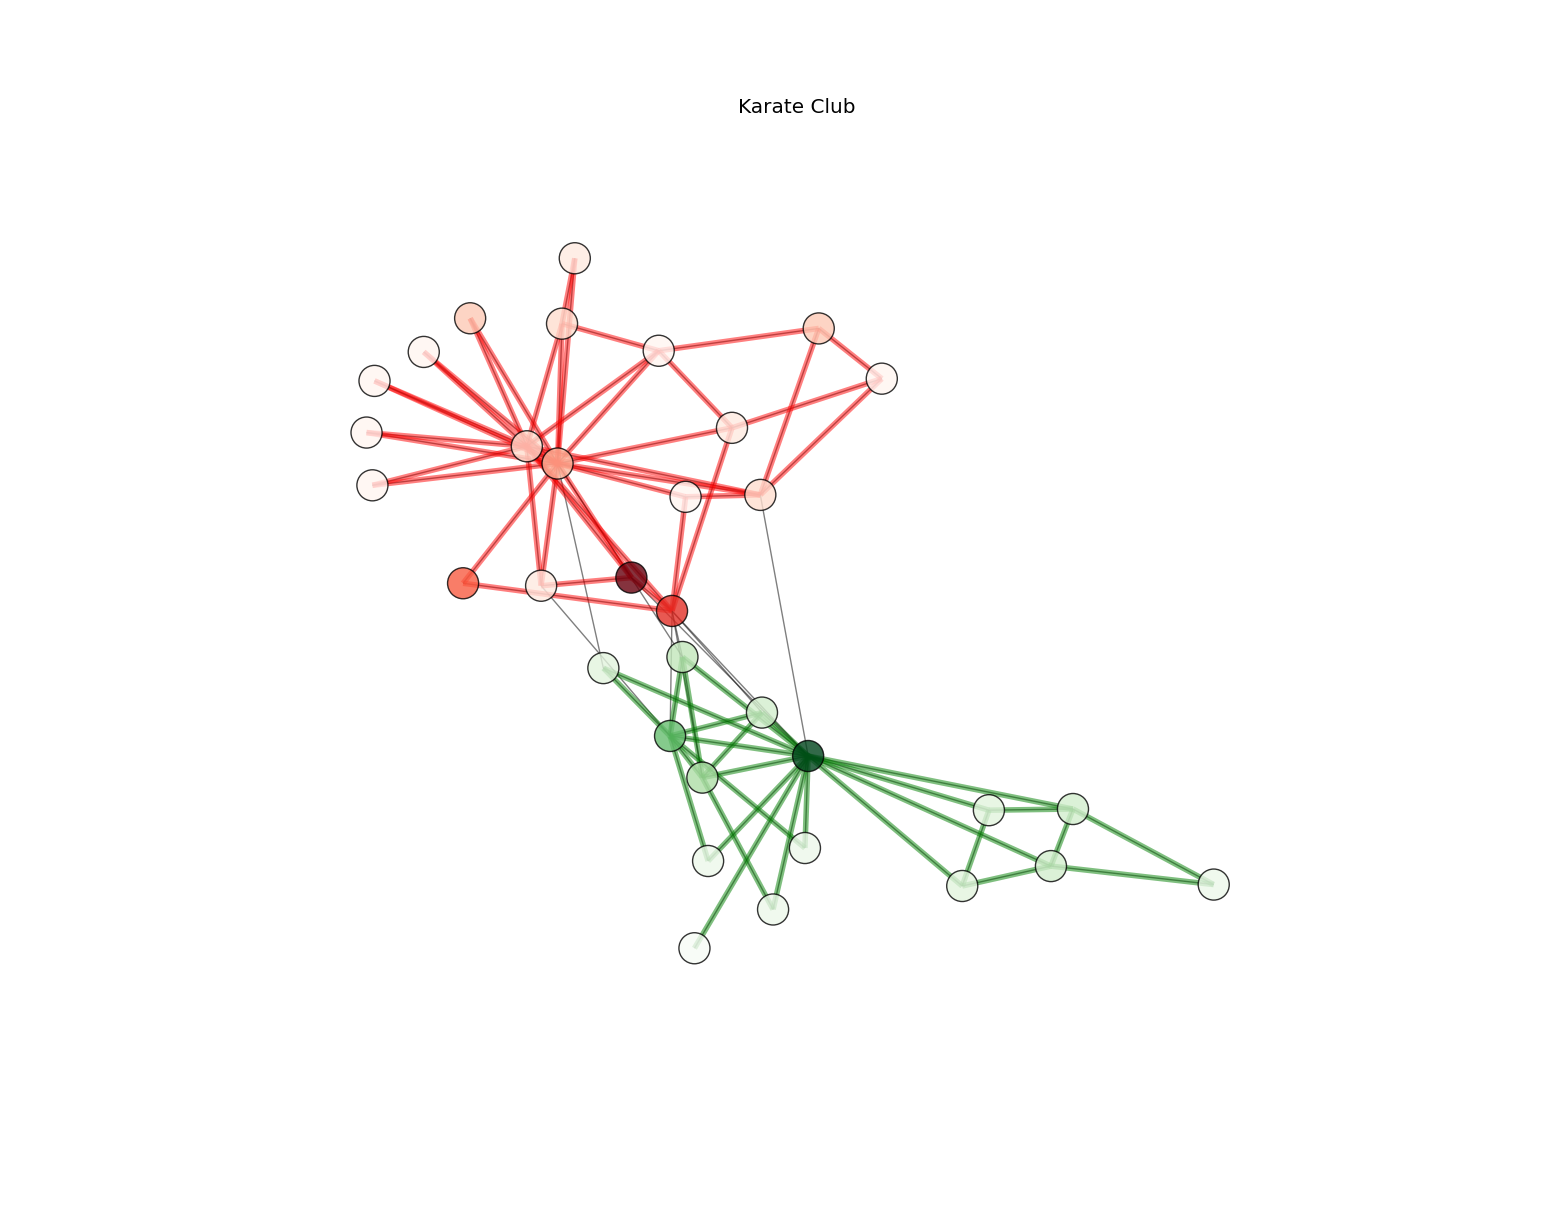
\includegraphics[width=.8\textwidth]{./figures/karate_club_split.png}
        \caption{Détection de communauté appliquée au club de karaté de
        Zachary.}
    \end{figure}
\end{frame}

\begin{frame}
    \frametitle{Approche spectrale}
    \begin{itemize}
        \item Méthode simple à implémenter
        \item Critère interprétable
        \item Condition d'arrêt
        \item Limites : coût en $\mathcal{O} (|V|^3)$, matrice de Laplace de
            taille $|V| \times |V|$
        \item Nécessité d'utiliser une méthode adaptée pour de grands réseaux
            (méthodes stochastiques)
    \end{itemize}
\end{frame}

\section{Génération dynamique de graphe}
\begin{frame}
    \begin{columns}
        \begin{column}{.5\textwidth}
            \begin{itemize}
                \item Graphe d'utilisateurs dynamique :
                    $\left( G_t = (V_t, E_t) \right)_{t \in \mathcal{T}}$
                \begin{itemize}
                    \item<2-> Nouveaux utilisateurs
                    \item<3-> Nouvelles connexions entre utilisateurs
                    \item<4-> Départ d'utilisateurs
                    \item<5-> Disparition de connexions
                    \item<6-> Évolution des connexions existantes (influence dynamique)
                \end{itemize}
            \end{itemize}
        \end{column}
        \begin{column}{.5\textwidth}
            \only<1>{
                \begin{figure}
                    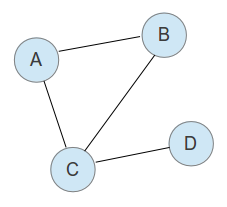
\includegraphics[width=.7\textwidth]{./figures/users_friendship.png}
                \end{figure}
            }
            \only<2>{
                \begin{figure}
                    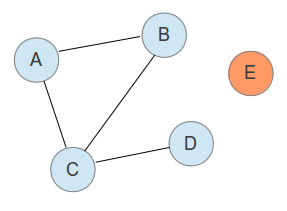
\includegraphics[width=.7\textwidth]{./figures/new_user.png}
                \end{figure}
            }
            \only<3>{
                \begin{figure}
                    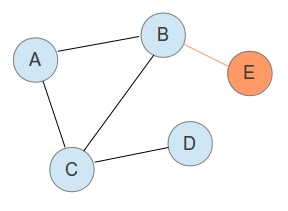
\includegraphics[width=.7\textwidth]{./figures/new_edge.png}
                \end{figure}
            }
            \only<4>{
                \begin{figure}
                    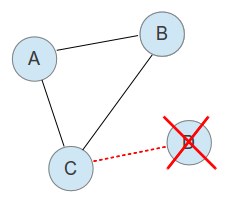
\includegraphics[width=.7\textwidth]{./figures/deleted_user.png}
                \end{figure}
            }
            \only<5-6>{
                \begin{figure}
                    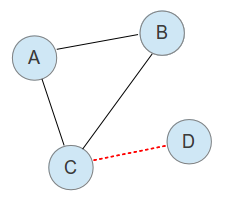
\includegraphics[width=.7\textwidth]{./figures/deleted_edge.png}
                \end{figure}
            }
        \end{column}
    \end{columns}
\end{frame}

\begin{frame}
        Peu de modèles existants sur graphes dynamique :
        \begin{itemize}
            \item Épidémiologie (théorie de la survie)
            \item Génétique (détection de \emph{pattern})
            \item Réseaux sociaux, web (citations, Internet)
        \end{itemize}
\end{frame}

\begin{frame}
    \frametitle{\emph{Community Guided Attachment}}

    \begin{itemize}
        \item Observations sur des graphes réels (réseaux sociaux, informatiques)
        \begin{itemize}
            \item Le degré moyen augmente quand le réseau grandit : $|E_t|
                \propto |V_t|^{\alpha}$, avec $1 < \alpha < 2$
        \end{itemize}
        \item Possible explication : connexions entre n\oe{}uds dépendantes
            des communautés
    \end{itemize}
\end{frame}

\begin{frame}
    \frametitle{\emph{Community Guided Attachment}}

    \begin{columns}
        \begin{column}{.5\textwidth}
            \begin{itemize}
                \item Structure des communautés en arbre (communautés dans les
                    communautés)
                \item Distance $h$ entre n\oe{}uds : distance dans l'arbre
            \end{itemize}
        \end{column}
        \begin{column}{.5\textwidth}
            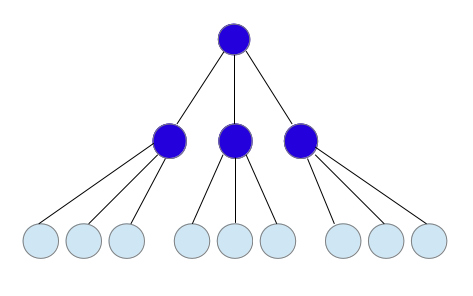
\includegraphics[width=.7\textwidth]{./figures/tree.png}
        \end{column}
    \end{columns}
\end{frame}

\begin{frame}
    \frametitle{\emph{Community Guided Attachment}}
    \begin{itemize}
        \item Nouveau n\oe{}ud $n_1$ se rattache à un n\oe{}ud $n_2$
            avec une probabilité $c^{d(n_1, n_2)}$
        \item Sous ce modèle, si arbre homogène de degré $b$, alors $|E|
            \propto |V|^{2 - \log_b(c)}$
    \end{itemize}
\end{frame}

\begin{frame}
    \begin{itemize}
        \item CGA donne une interprétation réaliste à un phénomène observé
        \item Mais ne se penche sur un seul aspect : pas d'effet \emph{small
            world}, pas de créations d'arrêtes parmi n\oe{}uds existants, etc.
        \item Nécessité de mixer les modèles
    \end{itemize}
\end{frame}

\begin{frame}
    \frametitle{Approche générale}
    \begin{itemize}
        \item Objectif : prédire l'évolution du graphe
        \item Définir un modèle d'évolution dynamique
        \item Utiliser l'historique des évolutions pour retrouver
            les paramètres du modèle
        \item Mettre à jour ces paramètres en ligne ou à intervalle fixé
    \end{itemize}
\end{frame}

\end{document}
